\section{Reverse-Mode Automatic Differentiation}\label{sec:reverse}

We briefly discuss the reverse-mode automatic differentiation algorithm
for context and to motivate the discussion for the next sections.
For a more in-depth treatment, we direct the readers 
to~\cite{carpenter:2015}\cite{margossian:2018}\cite{griewank:2008}.

As an example, consider the function 
\begin{equation}
    f(x_1, x_2, x_3) = \sin(x_1) + \cos(x_2) \cdot x_3 - \log(x_3)
    \label{eq:f-example}
\end{equation}
This function can be represented as an expression graph
where each node of the graph represents a sub-expression.
Fig.~\ref{fig:expr-example} shows the corresponding expression graph
drawn to evaluate in the same order as defined by the operator precedence in the C++ standard.

% Original expression graph
\begin{figure}[t]
\centering
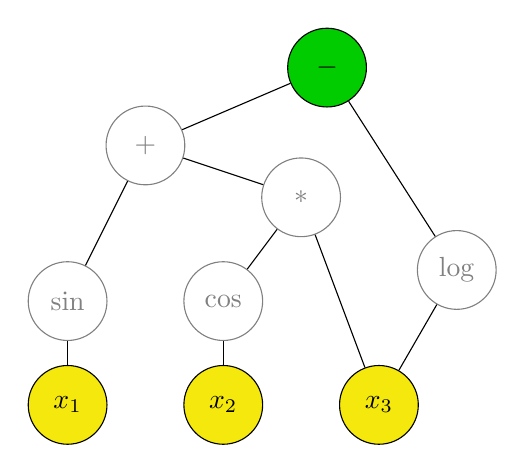
\begin{tikzpicture}[x=0.75pt,y=0.75pt,yscale=-0.5,xscale=0.5]

    \draw (150,350) node [align=center, minimum size=1cm, draw, circle, fill=black!5!yellow] (x1)  {$x_1$};
    \draw (300,350) node [align=center, minimum size=1cm, draw, circle, fill=black!5!yellow] (x2)  {$x_2$};
    \draw (450,350) node [align=center, minimum size=1cm, draw, circle, fill=black!5!yellow] (x3)  {$x_3$};
    \draw (150,250) node [align=center, minimum size=1cm, draw, circle, color=gray] (sin) {$\sin$};
    \draw (300,250) node [align=center, minimum size=1cm, draw, circle, color=gray] (cos) {$\cos$};
    \draw (525,220) node [align=center, minimum size=1cm, draw, circle, color=gray] (log) {$\log$};
    \draw (225,100) node [align=center, minimum size=1cm, draw, circle, color=gray] (add) {$+$};
    \draw (375,150) node [align=center, minimum size=1cm, draw, circle, color=gray] (mul) {$*$};
    \draw (400,25)  node [align=center, minimum size=1cm, draw, circle, fill=black!20!green] (sub) {$-$};
    \draw (x1) -- (sin);
    \draw (x2) -- (cos);
    \draw (x3) -- (mul);
    \draw (x3) -- (log);
    \draw (sin) -- (add);
    \draw (cos) -- (mul);
    \draw (mul) -- (add);
    \draw (add) -- (sub);
    \draw (log) -- (sub);

\end{tikzpicture}

\caption{Expression graph for Eq.~\ref{eq:f-example}}\label{fig:expr-example}

\end{figure}

Note that, in general, a variable $x_i$ can be referenced by multiple nodes.
For example, $x_3$ is referenced by the \code{*} and \code{log} nodes.
It is actually more helpful to convert this expression graph into an expression tree
by replacing all such nodes with multiple parents as separate nodes
that have a reference back to the actual variable.
Mathematically,
\begin{align}
    f(x_1, x_2, x_3) &= \tilde{f}(g(x_1, x_2, x_3)) \label{eq:f-tree-example} \\
    \tilde{f}(w_1, w_2, w_3, w_4) &= \sin(w_1) + \cos(w_2) \cdot w_3 - \log(w_4) \nonumber \\
    g(x_1, x_2, x_3) &= (x_1, x_2, x_3, x_3) \nonumber
\end{align}
Fig.~\ref{fig:expr-tree-example} shows the corresponding converted expression tree.
This way all nodes except possibly the \code{$x_i$} nodes have exactly one parent
and have a unique path back up to the root, if we view the tree as a directed graph.
While this may seem more complicated than the original expression graph,
implementation becomes much cleaner with this new approach.
With the converted expression tree, we will see momentarily that 
we may actually start the algorithm from $w_i$ instead of $x_i$.
In fact, rather than treating $x_i$ as nodes of the expression graph,
it is more helpful to instead treat them as containers 
that hold the initial values and their \textbf{adjoints}, $\frac{\partial f}{\partial x_i}$.
For this reason, we denote the path between $x_i$ and $w_i$ with dotted lines,
and consider only up to nodes $w_i$ in the expression tree.

% Converted expression tree
\begin{figure}[t]
\centering
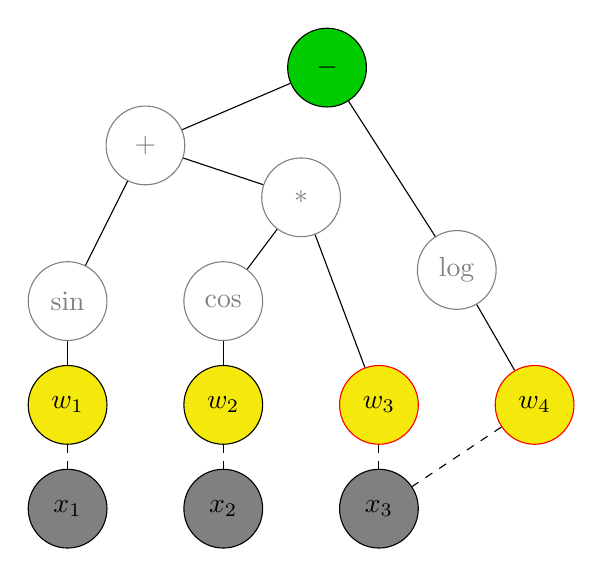
\begin{tikzpicture}[x=0.75pt,y=0.75pt,yscale=-0.5,xscale=0.5]

    \draw (150,450) node [align=center, minimum size=1cm, draw, circle, fill=gray] (x1)  {$x_1$};
    \draw (300,450) node [align=center, minimum size=1cm, draw, circle, fill=gray] (x2)  {$x_2$};
    \draw (450,450) node [align=center, minimum size=1cm, draw, circle, fill=gray] (x3)  {$x_3$};
    \draw (150,350) node [align=center, minimum size=1cm, draw, circle, fill=black!5!yellow] (w1)  {$w_1$};
    \draw (300,350) node [align=center, minimum size=1cm, draw, circle, fill=black!5!yellow] (w2)  {$w_2$};
    \draw (450,350) node [align=center, minimum size=1cm, draw=red, circle, fill=black!5!yellow] (w3)  {$w_3$};
    \draw (600,350) node [align=center, minimum size=1cm, draw=red, circle, fill=black!5!yellow] (w4)  {$w_4$};
    \draw (150,250) node [align=center, minimum size=1cm, draw, circle, color=gray] (sin) {$\sin$};
    \draw (300,250) node [align=center, minimum size=1cm, draw, circle, color=gray] (cos) {$\cos$};
    \draw (525,220) node [align=center, minimum size=1cm, draw, circle, color=gray] (log) {$\log$};
    \draw (225,100) node [align=center, minimum size=1cm, draw, circle, color=gray] (add) {$+$};
    \draw (375,150) node [align=center, minimum size=1cm, draw, circle, color=gray] (mul) {$*$};
    \draw (400,25)  node [align=center, minimum size=1cm, draw, circle, fill=black!20!green] (sub) {$-$};
    \draw [dashed] (w1) -- (x1);
    \draw [dashed] (w2) -- (x2);
    \draw [dashed] (w3) -- (x3);
    \draw [dashed] (w4) -- (x3);
    \draw (w1) -- (sin);
    \draw (w2) -- (cos);
    \draw (w3) -- (mul);
    \draw (w4) -- (log);
    \draw (sin) -- (add);
    \draw (cos) -- (mul);
    \draw (mul) -- (add);
    \draw (add) -- (sub);
    \draw (log) -- (sub);

\end{tikzpicture}

\caption{Converted expression tree for Eq.~\ref{eq:f-tree-example}.
         Nodes $x_1, x_2, x_3$ are now separated from the rest of the graph by a layer of $w$ variables.
         Note in particular that $x_3$ is now replaced with $w_3$ and $w_4$ (red boundary).
}\label{fig:expr-tree-example}

\end{figure}

The reverse-mode algorithm consists of two passes of the expression graph:
\emph{forward}-evaluation (not to be confused with forward-mode AD), 
and \emph{backward}-evaluation.
During the \emph{forward}-evaluation, we compute the expression in the usual fashion,
i.e.\ start at the root, recursively forward-evaluate from left to right all of its children,
then finally take those results and evaluate the current node.
Evaluation of each node will compute the operation that it represents.
For example, after forward-evaluating the $w_1$ node, 
which is a trivial operation of retrieving the value from the container $x_1$,
the \code{sin} node will return~$\sin(w_1) = \sin(x_1)$.

The \emph{backward}-evaluation for a given node starts by receiving its adjoint from its parent.
We will also refer to this value as its \emph{seed} to further distinguish $x_i$ from the expression nodes.
Since the seed is exactly the partial derivative of $f$ with respect to the node,
the root of the expression tree will receive the value $ \frac{\partial f}{\partial f} = 1$.
Using the seed, the node computes the correct seed for all of its children and 
backward-evaluates from \emph{right-to-left}, the opposite direction of forward-evaluation.

The correct seed for each child is computed by a simple chain-rule.
Assuming the current node is represented by $w \in \R$ and one of its children is $v \in \R$,
the seed for $v$ is the following:
\begin{align}
    \frac{\partial f}{\partial v} &=
    \frac{df}{dw} \frac{\partial w}{\partial v} \label{eq:next-seed}
\end{align}
Each node $w$ has node-specific information to compute $\frac{\partial w}{\partial v}$.
For example, for the \code{log} node in Fig.~\ref{fig:expr-tree-example},
with $w$ as \code{log} and $v$ as $w_4$,
\begin{align*}
    \frac{\partial w}{\partial v} = \frac{d\log(w_4)}{dw_4} = \frac{1}{w_4}
\end{align*}
In general, if $v \in \R^{m \times n}$ and $w \in \R^{p \times q}$, then
\begin{align}
    \frac{\partial f}{\partial v_{ij}} &=
        \sum\limits_{k=1}^p \sum\limits_{l=1}^q 
        \frac{\partial f}{\partial w_{kl}} \frac{\partial w_{kl}}{\partial v_{ij}}
    \label{eq:next-adj}
\end{align}
In particular, the adjoint will always have the same shape and size as the value.

For nodes that have references back to the containers $x_i$, i.e.\ $w_1,\ldots,w_4$,
they must increment the adjoints in the containers with their seeds.
For example, nodes $w_3$ and $w_4$ will take their seeds and increment the adjoint for $x_3$.
This is easily seen by chain-rule again: let~$w_1, \ldots, w_k$ denote all of the variables that 
references $x$ and for simplicity assume they are all scalar, 
although the result can be easily generalized for multiple dimensions.
Then,
\begin{align*}
    \frac{\partial f}{\partial x} 
    &=  \sum\limits_{i=1}^k
        \frac{\partial f}{\partial w_{i}} \frac{\partial w_{i}}{\partial x}
    =   \sum\limits_{i=1}^k
        \frac{\partial f}{\partial w_{i}}
\end{align*}
where $\frac{\partial w_i}{\partial x} = 1$ because $w_i$ is simply the identity function with respect to $x$.
The fully accumulated adjoints for $x_1, x_2, x_3$ form the gradient of $f$.

In general, an expression node can be quite general and 
is only required to define how to compute its value and 
the adjoints of its children using Eq.~\ref{eq:next-adj}.

In the general case where $f: \R^n \to \R^m$,
we can apply this algorithm for the scalar functions $f_j$ for $j = 1,\ldots,m$ and
save each gradient as the $j$th row of a matrix.
The final matrix is then the Jacobian of $f$.
